\documentclass[12pt]{beamer}
%\documentclass[20pt,handout]{beamer}
\usetheme{Darmstadt}
\usepackage{graphicx}
%\usepackage[german]{babel}
\usepackage{ngerman}
\usepackage[T1]{fontenc}
\usepackage[utf8]{inputenc}
\usepackage{tikz}
\setbeamertemplate{footline}[frame number]

\newcommand{\cc}[1]{\includegraphics[height=4mm]{img/#1.png}\hspace{1mm}}
\usepackage{ifthen}
\newcommand{\license}[2][]{\\#2\ifthenelse{\equal{#1}{}}{}{\\\scriptsize\url{#1}}}
\usepackage{textcomp}
\usepackage{hyperref}

\pgfdeclareimage[height=.6cm]{c3d2logo}{./img/c3d2.pdf} 


\pgfdeclarelayer{foreground}
\pgfsetlayers{main,foreground}
\logo{\pgfputat{\pgfxy(-1,0)}{\pgfbox[center,base]{\pgfuseimage{c3d2logo}}}}


\title{NSA, Prism und co - Wie schützt man sich vor Überwachung?}
\author{\small Stefan Böcker, Martin Byrenheid, Marius Melzer\\\large Chaos Computer Club Dresden}
\date{20.05.2014}

\begin{document}
\maketitle

\section{CCC}
\subsection{}

\begin{frame}
  \frametitle{Chaos Computer Club}
  \begin{figure}
    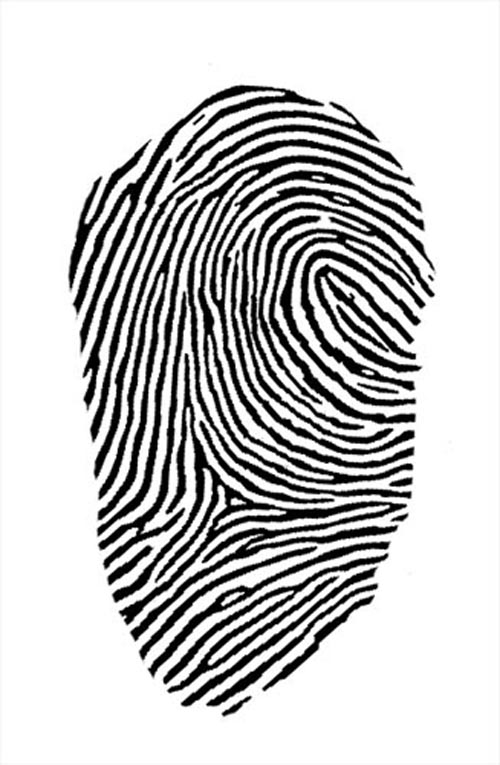
\includegraphics[height=0.7\textheight]{img/fingerabdruck.jpg}
  \end{figure}
\end{frame}

\begin{frame}
  \frametitle{Chaos Computer Club}
  \begin{figure}
    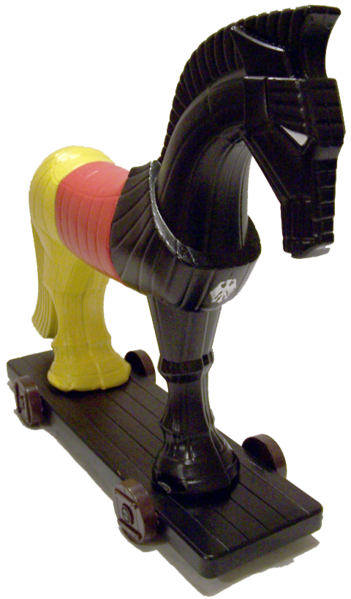
\includegraphics[height=0.7\textheight]{img/trojaner.png}
  \end{figure}
\end{frame}

\begin{frame}
    \frametitle{Chaos Computer Club}
    \begin{itemize}
      \item<1-> Chaos Computer Club Dresden (\url{http://c3d2.de})
          \note{}
      \item<2-> Datenspuren: 13./14.09.2014 \url{http://datenspuren.de}
      \item<3-> Podcasts (\url{http://pentamedia.de})
      \item<4-> Chaos macht Schule
    \end{itemize}
\end{frame}

\begin{frame}
    \frametitle{Bundespräsident Gauck zur NSA-Überwachung}
    \begin{center}
      ``Wir wissen z.B., dass es nicht so ist, wie bei der Stasi und dem KGB, dass es dicke Aktenbände gibt, wo unsere Gesprächsinhalte alle aufgeschrieben und schön abgeheftet sind. Das ist es nicht.''
      \end{center}
\end{frame}

\begin{frame}
    \frametitle{Stasi vs. NSA}
    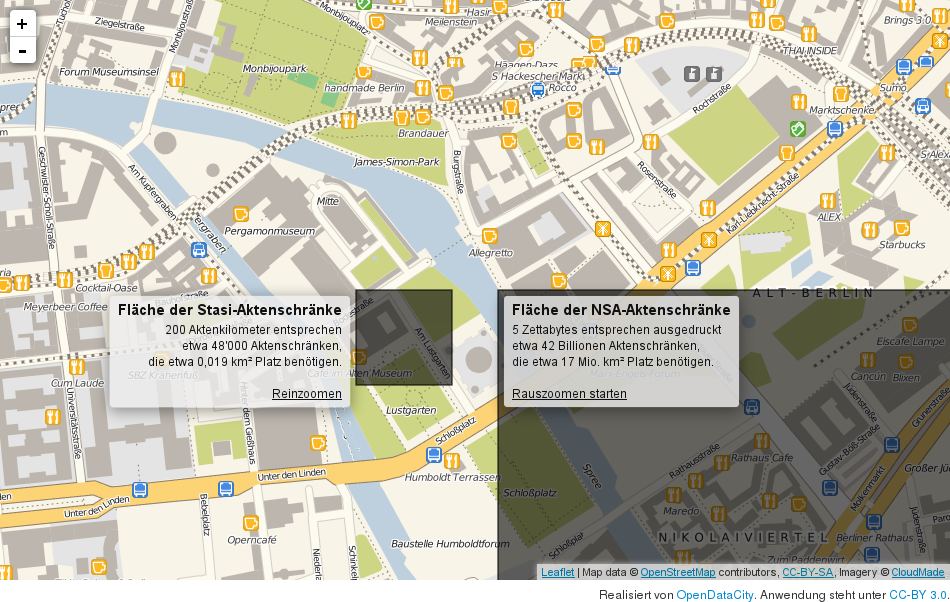
\includegraphics[height=0.7\textheight]{img/akten1.png}
\end{frame}

\begin{frame}
    \frametitle{Stasi vs. NSA}
    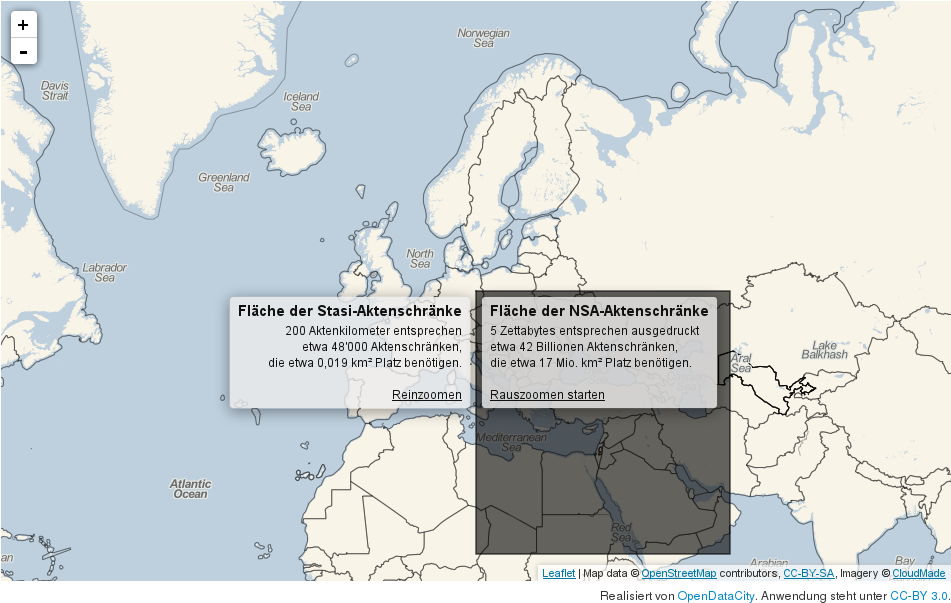
\includegraphics[height=0.7\textheight]{img/akten2.png}
\end{frame}

\begin{frame}
    \frametitle{Merkels Handy}
    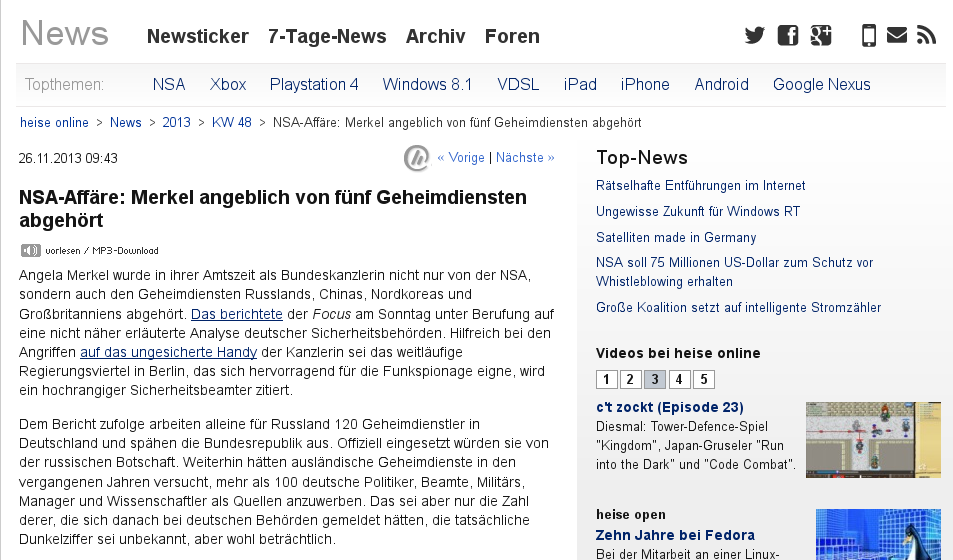
\includegraphics[height=0.7\textheight]{img/heise-merkel.png}
\end{frame}


\begin{frame}
    \frametitle{NSA-Skandal}
    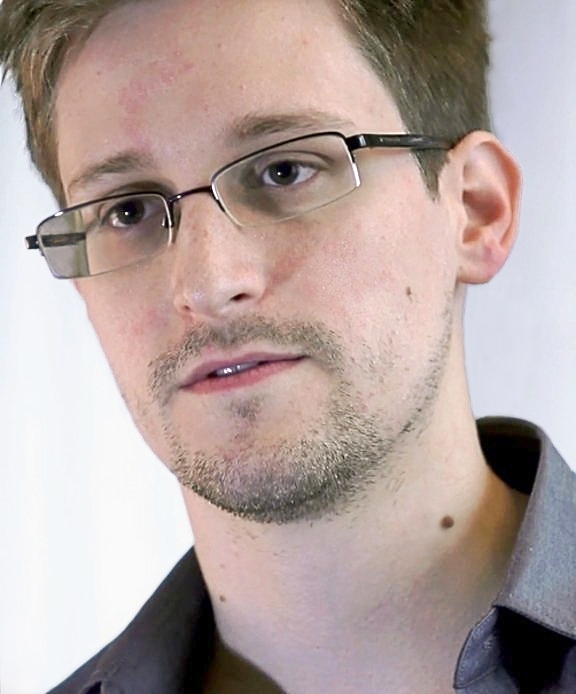
\includegraphics[height=0.7\textheight]{img/snowden.jpg}
    \\{\small \href{https://commons.wikimedia.org/wiki/File:Edward_Snowden.jpg\#mediaviewer/File:Edward_Snowden-2.jpg}{Grafik}: \href{https://creativecommons.org/licenses/by/3.0/}{\cc{by}} Laura Poitras / Praxis Films}
\end{frame}

\section{Kommunikation}
\subsection{}

\begin{frame}
    \frametitle{Tempora}
    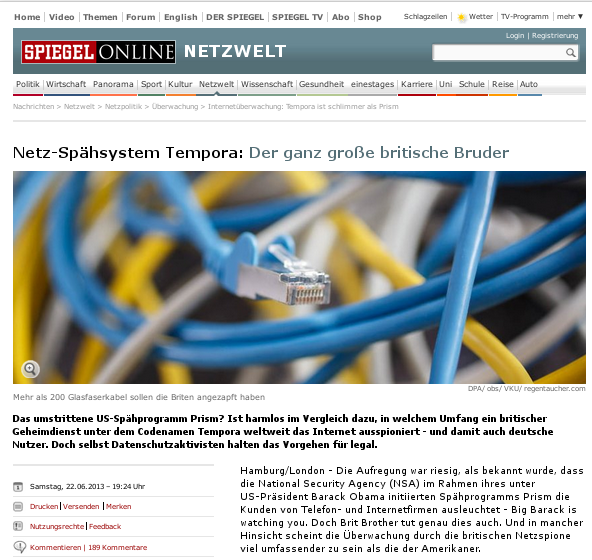
\includegraphics[height=0.7\textheight]{img/spiegel-tempora.png}
\end{frame}

\begin{frame}
    \frametitle{Mail}
    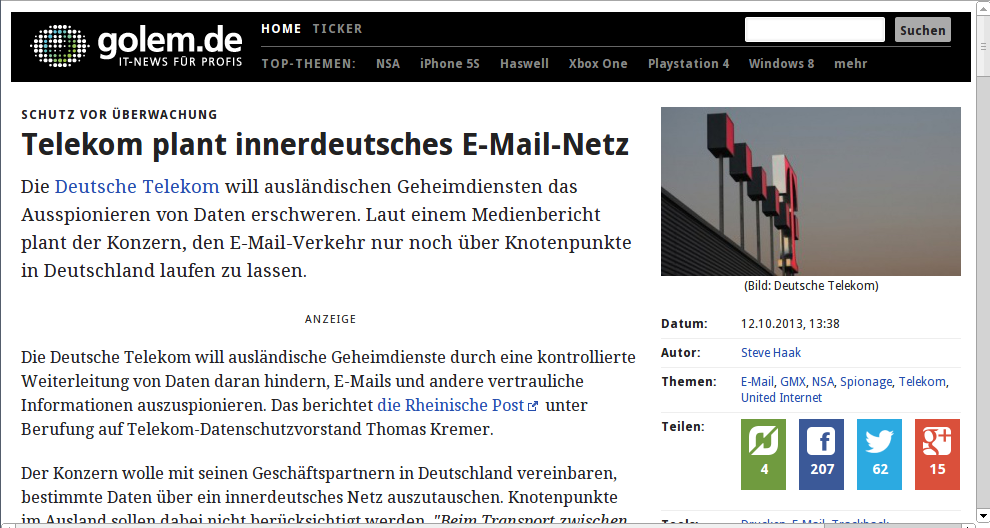
\includegraphics[height=0.7\textheight]{img/telekom_mail.png}
\end{frame}

\begin{frame}
    \frametitle{Verschlüsselung: Analogie}
    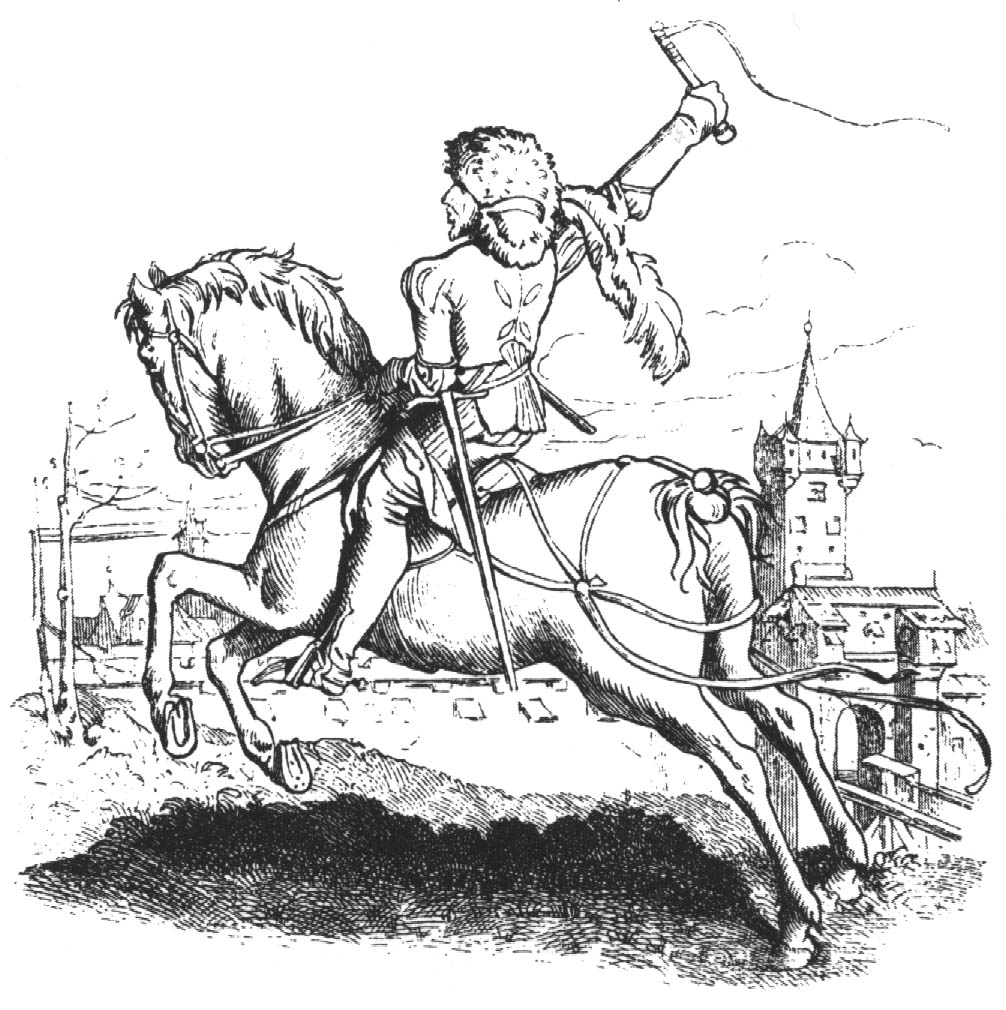
\includegraphics[height=0.7\textheight]{img/bote.jpg}
    {\\ \small \href{http://commons.wikimedia.org/wiki/File:Reitbote.jpg}{Grafik}: \href{http://creativecommons.org/licenses/by-sa/2.5/deed.en}{\cc{by-sa}} Ronald Preuss}
\end{frame}

\begin{frame}
    \frametitle{Verschlüsselung: Asymmetrische}
    \includegraphics[height=0.7\textheight]<2->{img/asym_encryption.png}
\end{frame}

\begin{frame}
    \frametitle{SSL / TLS}
    \begin{itemize}
      \item<2-> SSL = Secure Socket Layer
      \item<3-> eingesetzt im Web, Mail, ...
      \item<4-> hierarchische Struktur
    \end{itemize}
\end{frame}

\begin{frame}
    \frametitle{SSL im Browser}
    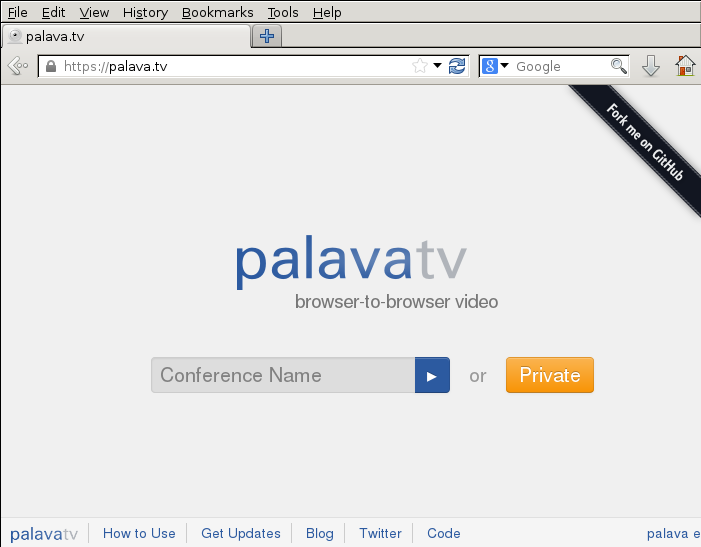
\includegraphics[height=0.7\textheight]{img/ssl_verified.png}
\end{frame}

\begin{frame}
    \frametitle{SSL im Browser}
    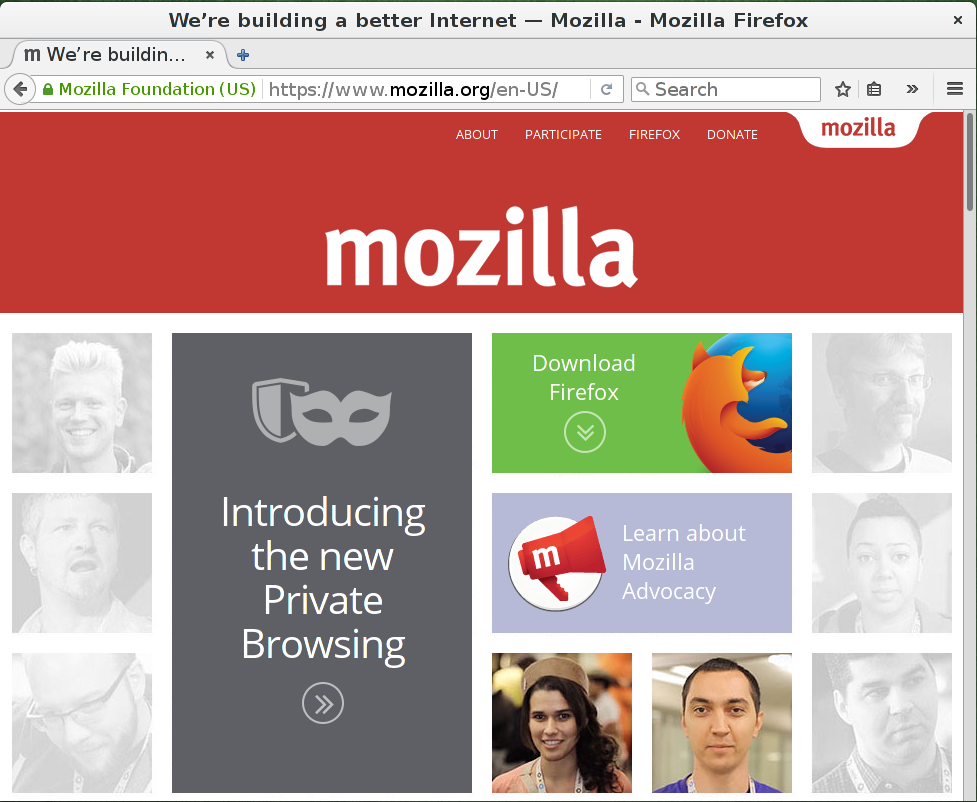
\includegraphics[height=0.7\textheight]{img/ssl_special.png}
\end{frame}

\begin{frame}
    \frametitle{SSL im Browser}
    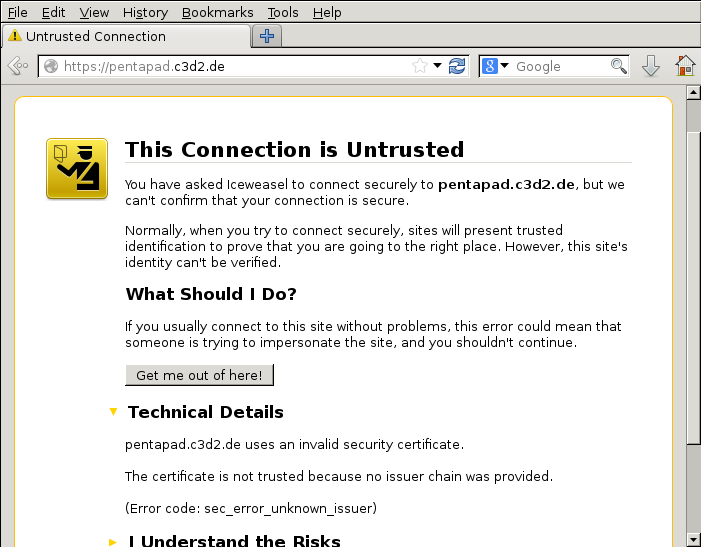
\includegraphics[height=0.7\textheight]{img/ssl_unverified.png}
\end{frame}

\begin{frame}
    \frametitle{Zertifizierungsstellen}
    \begin{center}
      \includegraphics[height=5cm]<2->{img/zertifikate.png}
    \end{center}
\end{frame}

\begin{frame}
  \frametitle{HTTPS Everywhere}
    \begin{center}
      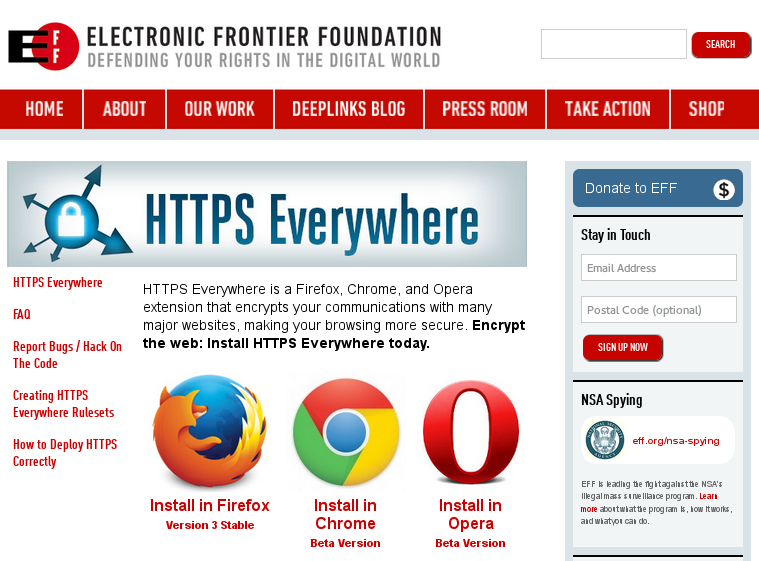
\includegraphics[height=5cm]{img/https-everywhere.png}
    \end{center}
\end{frame}
%% http://www.theconnectivist.com/2013/06/the-expanding-consolidation-of-the-consumer-internet/

\section{Inhalte}
\subsection{}

\begin{frame}
    \frametitle{Prism}
    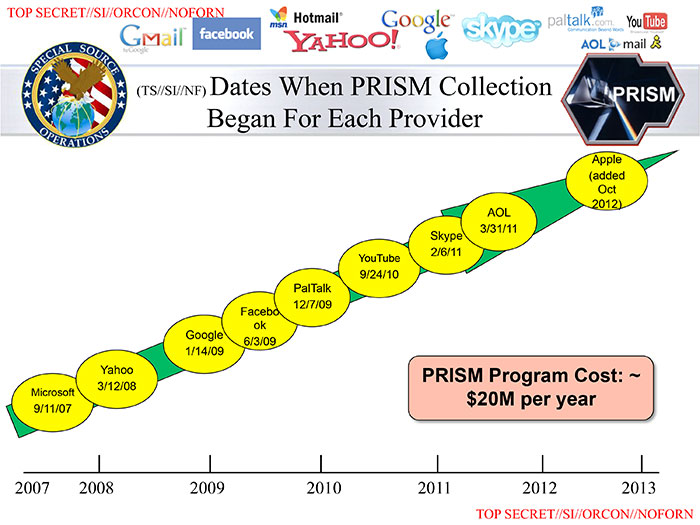
\includegraphics[height=0.7\textheight]{img/prism.jpg}
\end{frame}

\begin{frame}
  \frametitle{Dezentrale Dienste}
    \begin{columns}
        \begin{column}{5cm}
            \begin{center}
                
\includegraphics[height=0.2\textheight]{img/mail.pdf} \\
                E-Mail \\
                \vspace{1cm}
                
\includegraphics[height=0.2\textheight]{img/jabber.png}
            \end{center}
        \end{column}
        \begin{column}{5cm}
            \begin{center}
                
\includegraphics[height=0.2\textheight]{img/bitmessagelogo.png} \\
                Bitmessage \\
                \vspace{1cm}
                
\includegraphics[width=0.8\textwidth]{img/palava-tv.png}
            \end{center}
        \end{column}
    \end{columns}
\end{frame}

\begin{frame}
    \frametitle{Lavabit}
    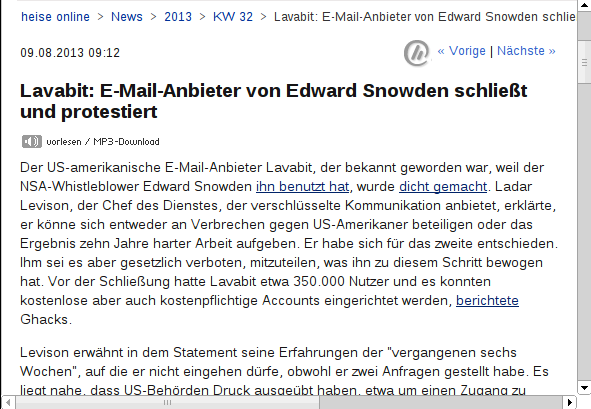
\includegraphics[height=0.6\textheight]{img/heise_lavabit.png}
\end{frame}

\begin{frame}
    \frametitle{Ende-zu-Ende-Verschlüsselung I}
    \begin{itemize}\Large
      \item Email: GPG = Gnu Privacy Guard
      \item Thunderbird: Enigmail
      \item Outlook: Gpg4win
      \item Apple Mail: GPGTools
      \item Web: Mailvelope (Firefox, Chrome)
    \end{itemize}
\end{frame}

\begin{frame}
  \frametitle{Ende-zu-Ende-Verschlüsselung II}
  \begin{itemize}
    \item<2-> OTR für Jabber:
      \begin{itemize}
        \item Pidgin mit OTR-Plugin für Linux und Windows
        \item GibberBot oder Xabber für Android
        \item Adium für Mac, ChatSecure für iOS
      \end{itemize}
    \item<3-> palava.tv für Videotelefonie
    \item<4-> Redphone für Handytelefonate (Android)
    \item<5-> TextSecure für Nachrichten (Android)
  \end{itemize}
\end{frame}

\begin{frame}
  \frametitle{Authentifizierung}
    \begin{center}
      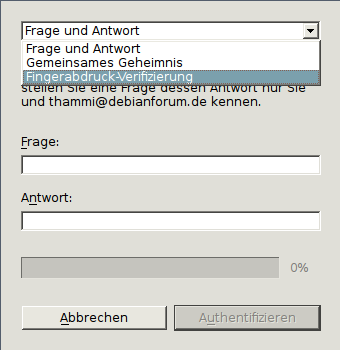
\includegraphics[height=5cm]{img/auth.png}
    \end{center}
\end{frame}

\begin{frame}
  \frametitle{TextSecure}
    \begin{center}
      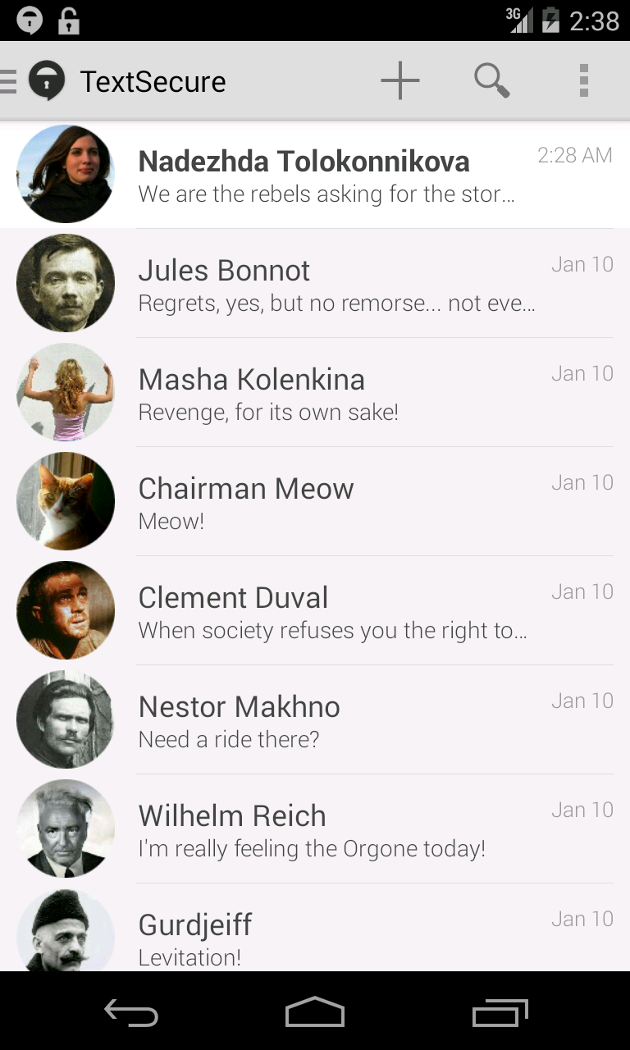
\includegraphics[height=6cm]{img/textsecure1.png}
      \hspace{0.5cm}
      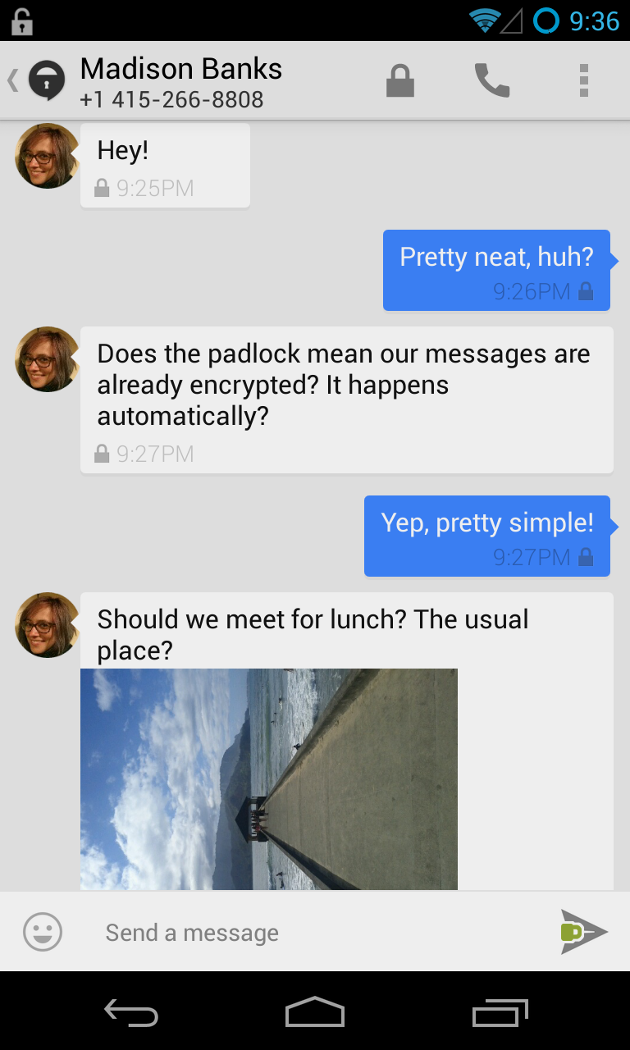
\includegraphics[height=6cm]{img/textsecure2.png}
    \end{center}
\end{frame}
 
\section{Metadaten}
\subsection{}

\begin{frame}
  \frametitle{Metadaten}
  \begin{itemize}
    \item Handynetz
      \begin{itemize}
        \item Telefonnummern
        \item Zeitpunkt und Dauer (Telefonate, SMS)
        \item Funkzelle (Ort)
      \end{itemize}
    \item Internet
      \begin{itemize}
        \item IP-Adresse
        \item Alle Verbindungen
        \item Email: Adressen von Sender und Empfänger, Zugriff
      \end{itemize}
  \end{itemize}
\end{frame}

\begin{frame}
  \frametitle{Vorratsdatenspeicherung (USA)}
    \begin{center}
      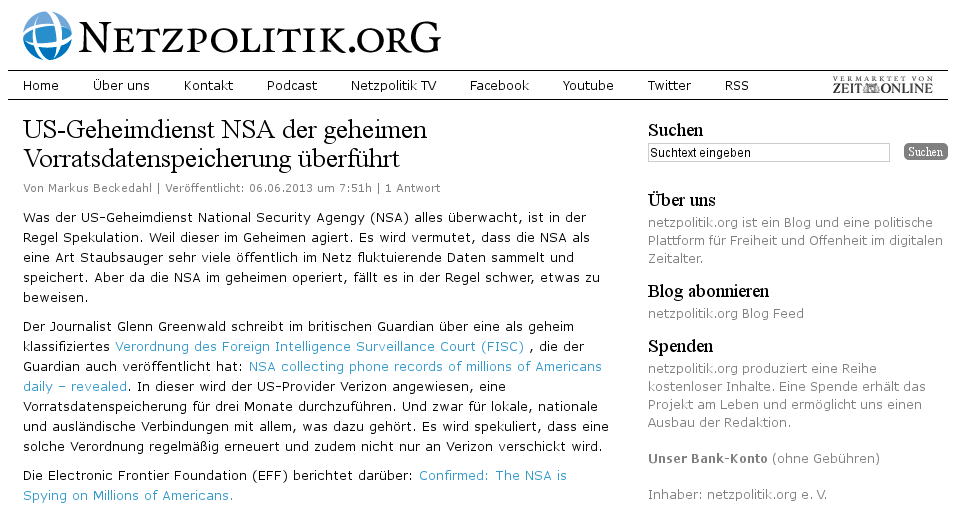
\includegraphics[height=5cm]{img/netzpolitik-verizon.png}
    \end{center}
\end{frame}

\begin{frame}
  \frametitle{Vorratsdatenspeicherung (Deutschland)}
    \begin{center}
      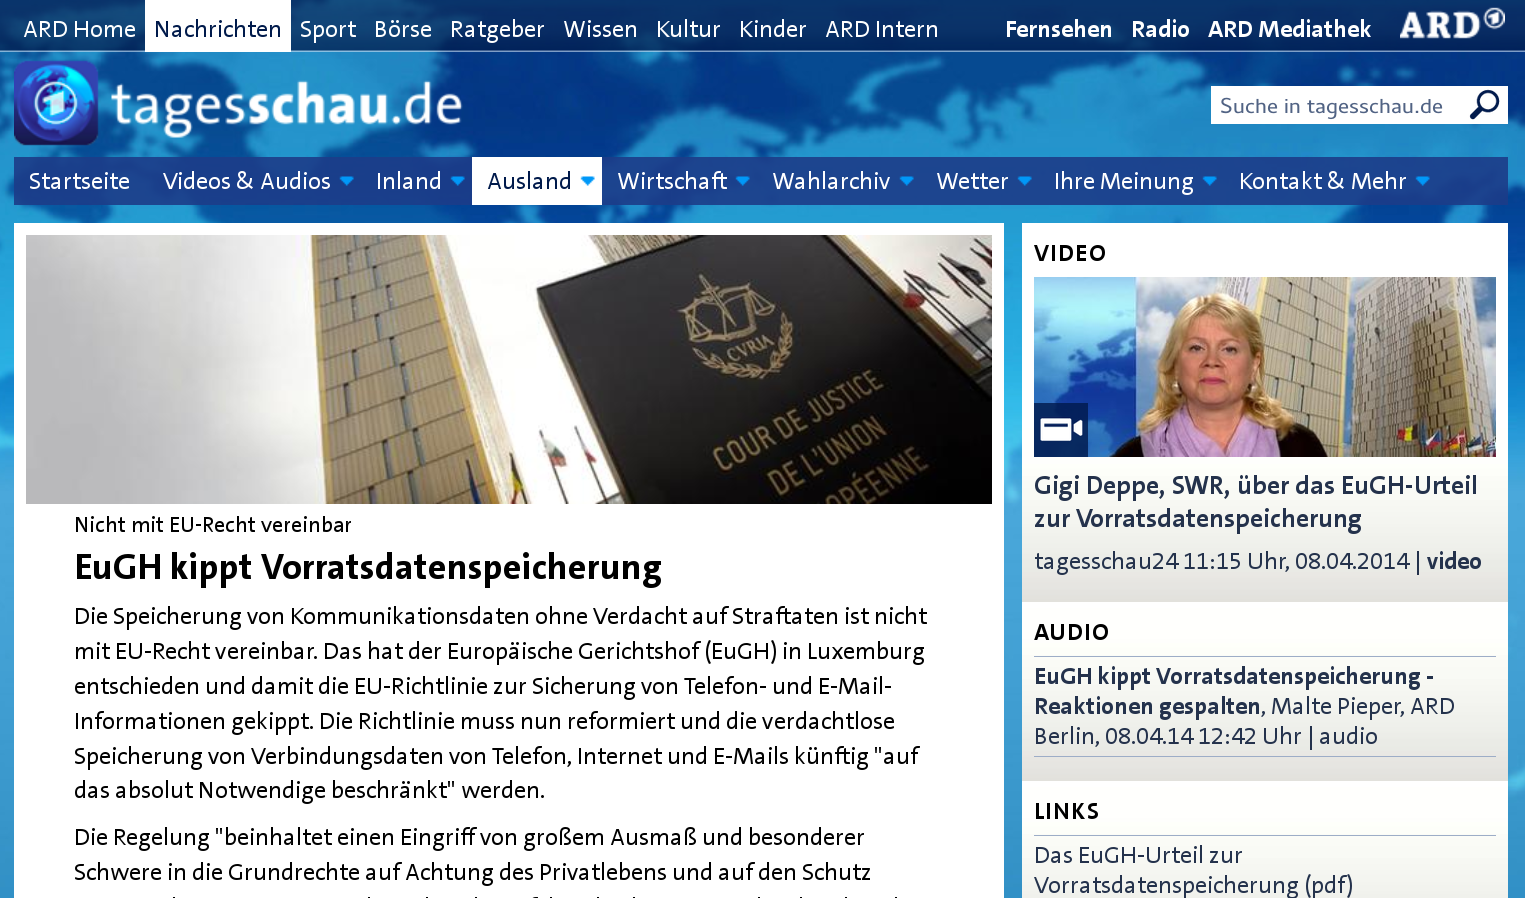
\includegraphics[height=5cm]{img/tagesschau-vds.png}
    \end{center}
\end{frame}

\begin{frame}
  \frametitle{Metadaten}
    \begin{center}
      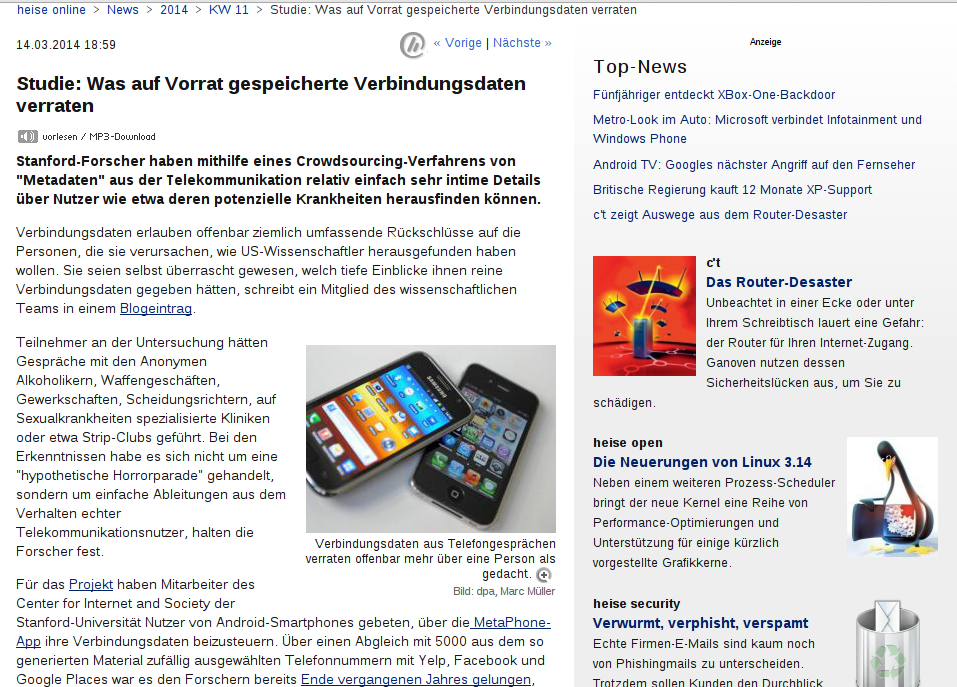
\includegraphics[height=5cm]{img/metadaten_studie.png}
    \end{center}
\end{frame}

\begin{frame}
    \frametitle{Metadaten}
    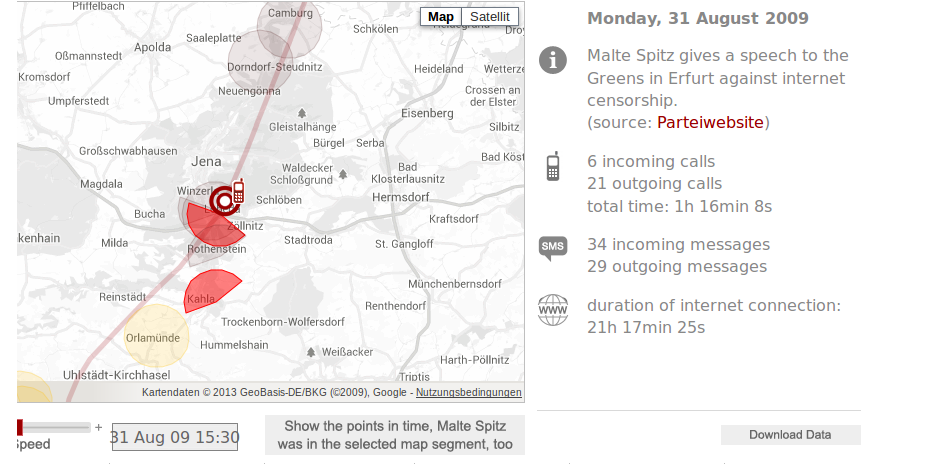
\includegraphics[height=0.7\textheight]{img/maltespitz.png}
\end{frame}

\begin{frame}
    \frametitle{Metadaten}
    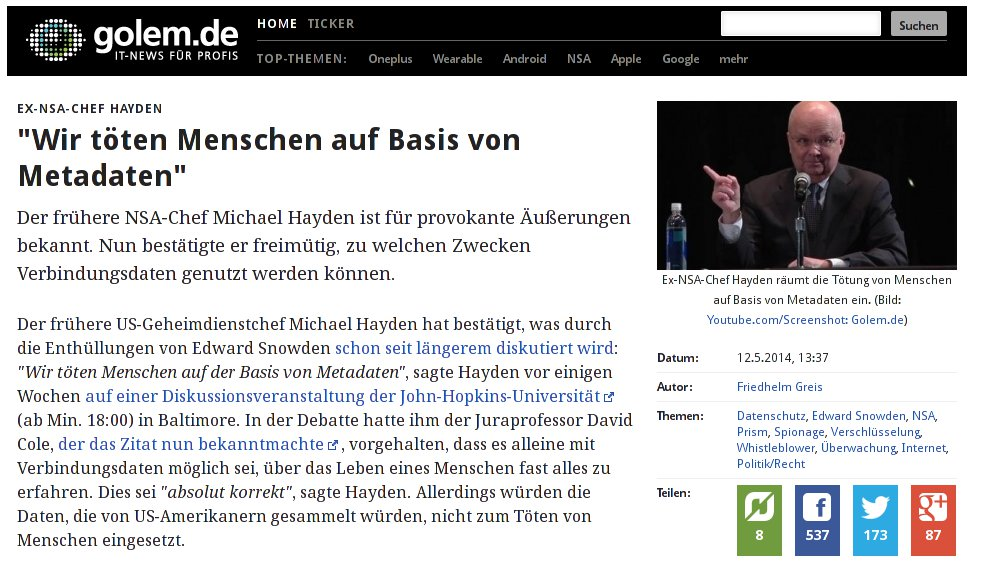
\includegraphics[height=0.7\textheight]{img/wekillpeople.jpg}
\end{frame}

\begin{frame}
    \frametitle{Tor}
    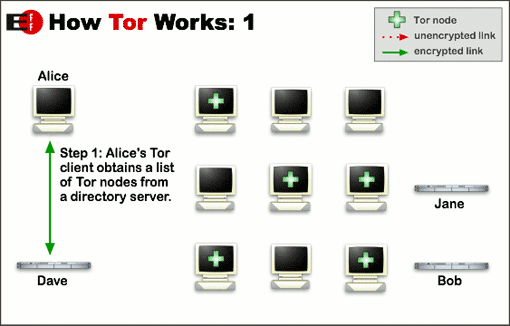
\includegraphics[height=0.7\textheight]{img/tor1.png}
    \\{\small \href{https://www.torproject.org/images/htw1.png}{Grafik}: \href{https://creativecommons.org/licenses/by/3.0/us/}{\cc{by}} The Tor Project}
\end{frame}

\begin{frame}
    \frametitle{Tor}
    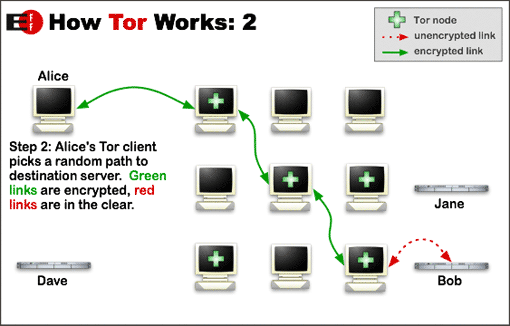
\includegraphics[height=0.7\textheight]{img/tor2.png}
    \\{\small \href{https://www.torproject.org/images/htw2.png}{Grafik}: \href{https://creativecommons.org/licenses/by/3.0/us/}{\cc{by}} The Tor Project}
\end{frame}

\begin{frame}
    \frametitle{Tor}
    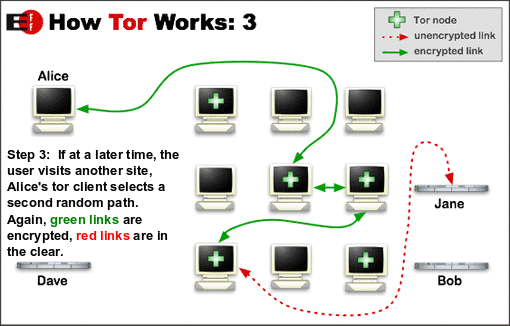
\includegraphics[height=0.7\textheight]{img/tor3.png}
    \\{\small \href{https://www.torproject.org/images/htw3.png}{Grafik}: \href{https://creativecommons.org/licenses/by/3.0/us/}{\cc{by}} The Tor Project}
\end{frame}

\begin{frame}
  \frametitle{Tor}
  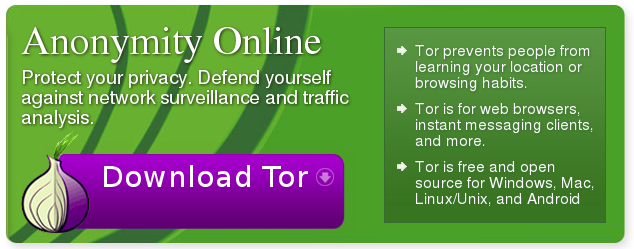
\includegraphics[height=0.5\textheight]{img/tor-banner.png}
\end{frame}

%%\begin{frame}
%%    \frametitle{Zensur}
%%    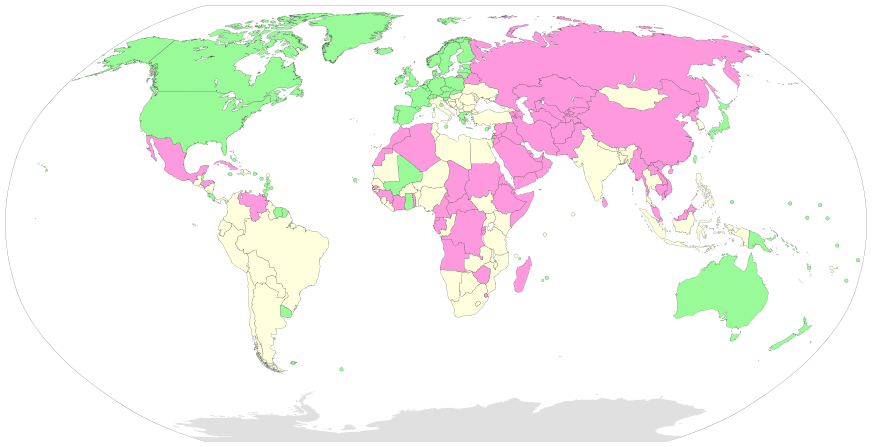
\includegraphics[height=0.7\textheight]{img/zensur.png}
%%    \\{\small \href{http://upload.wikimedia.org/wikipedia/commons/5/51/RWB-PressFreedomIndex2013-WorldMap.svg}{Grafik}: \href{http://creativecommons.org/licenses/by-sa/3.0/deed.en}{\cc{by-sa}} Jeff Ogden (W163)}
%%\end{frame}

\begin{frame}
    \frametitle{Tor in Deutschland}
    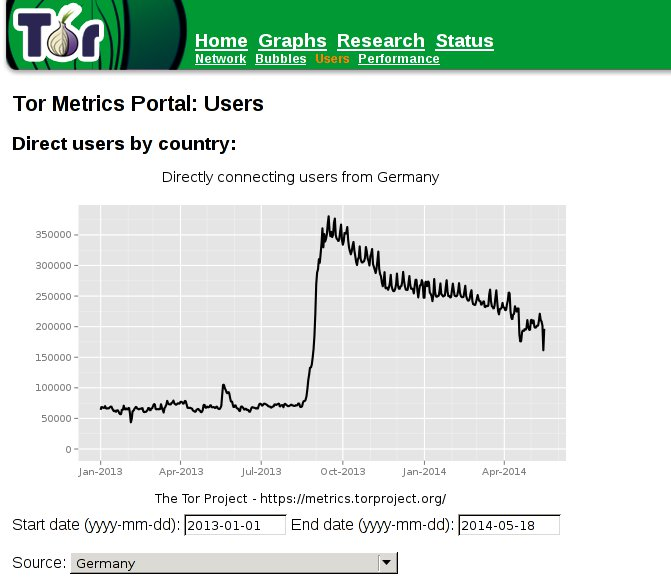
\includegraphics[height=0.7\textheight]{img/torgermany.jpg}
\end{frame}

\begin{frame}
    \frametitle{Anonymität unter Vollüberwachung}
    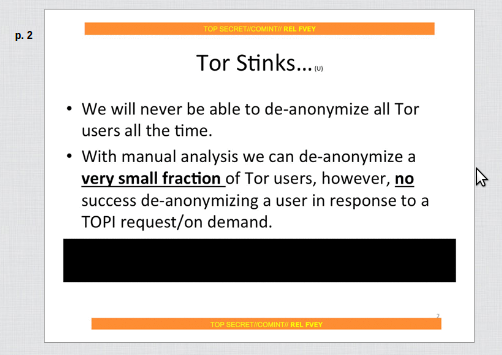
\includegraphics[height=0.7\textheight]{img/torstinks.png}
\end{frame}

% =================== Ende Stephan, Anfang Marius =================

\begin{frame}
    \frametitle{Metadaten - Lightbeam}
    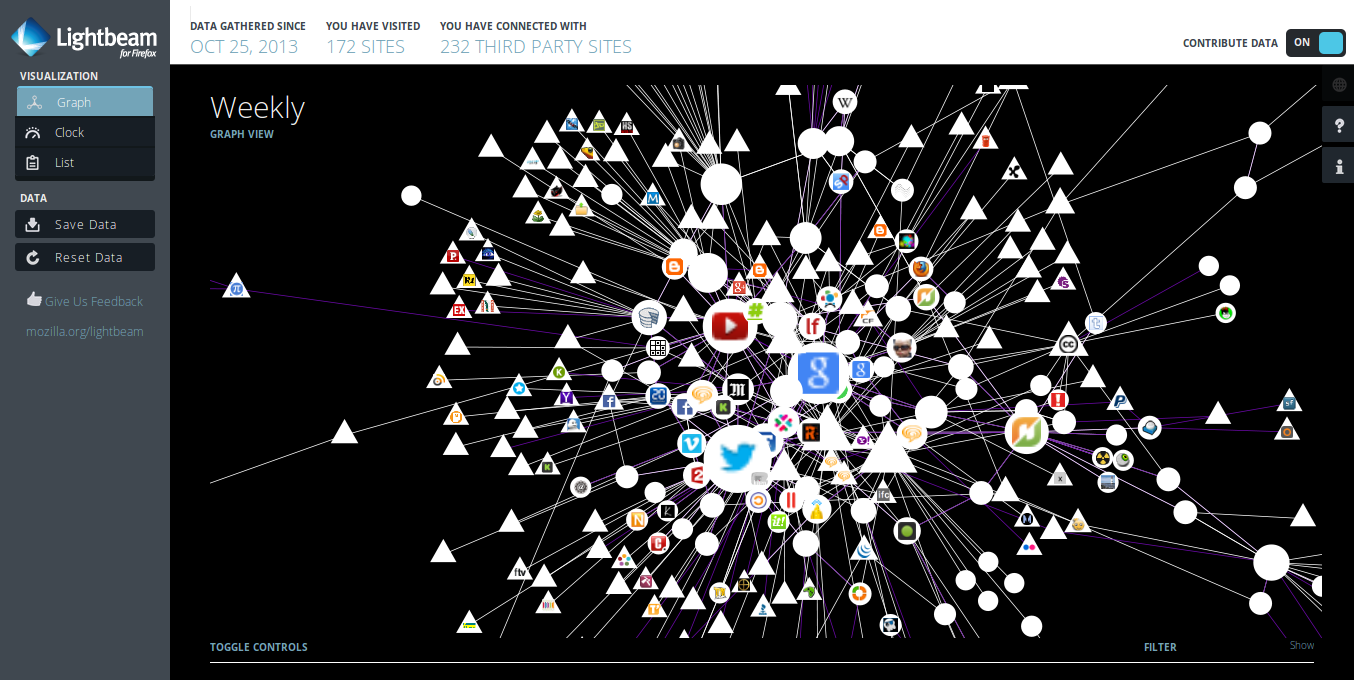
\includegraphics[height=0.7\textheight]{img/lightbeam.png}
  \\{\small \href{http://www.flickr.com/photos/8517757@N03/10538205035/in/photolist-h4e4dg}{Grafik:} \href{http://creativecommons.org/licenses/by-sa/3.0/deed.en}{\cc{by-sa}} Clint Lalonde}
\end{frame}

\begin{frame}
  \frametitle{Metadaten - Disconnect}
  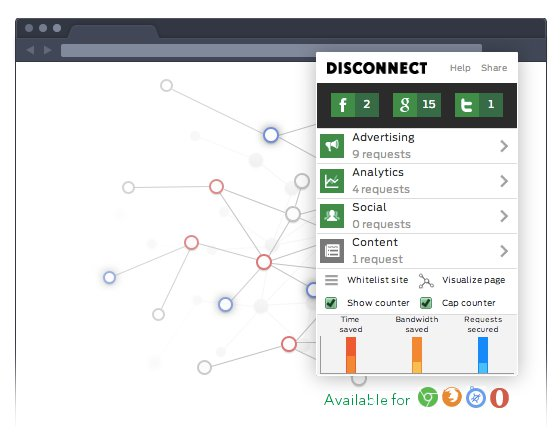
\includegraphics[height=0.7\textheight]{img/disconnectme.jpg}
\end{frame}


\section{Freie Software}
\subsection{}

\begin{frame}
  \frametitle{Kompilierung von Software}
  \begin{center}
    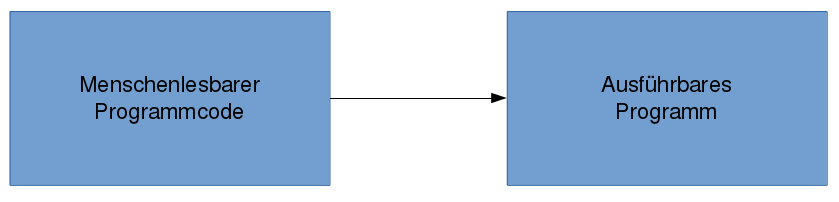
\includegraphics[width=10cm]{img/compilation-process}
  \par\end{center}
\end{frame}

\begin{frame}
  \frametitle{Probleme von proprietärer Software}
  \begin{itemize}
    \item<2-> Kontrolle unterliegt einer Organisation
    \item<3-> Transparenz und Sicherheit
  \end{itemize}
\end{frame}

\begin{frame}
  \frametitle{Strategien moderner IT-Unternehmen}
  \begin{itemize}
    \item<2-> Hardware
    \item<3-> Software
    \item<4-> Internetdienste
    \item<5-> ... aus einer Hand
  \end{itemize}
\end{frame}

\begin{frame}
  \frametitle{Strategien moderner IT-Unternehmen}
  \begin{itemize}
    \item<2-> Fehlende Interoperabilität
    \item<3-> vorgegebene Dienste und Programme
    \item<4-> keine ausreichenden Nutzerrechte
    \item<5-> Kopierschutz, Online-Zwang, ...
  \end{itemize}
\end{frame}

\begin{frame}
  \frametitle{Strategien moderner IT-Unternehmen}
  \begin{center}
    ``Tie all of our products together, so we further lock customers into our ecosystem'' (Steve Jobs)
  \end{center}
\end{frame}

\begin{frame}
  \frametitle{Backdoors in Windows}
  \begin{center}
    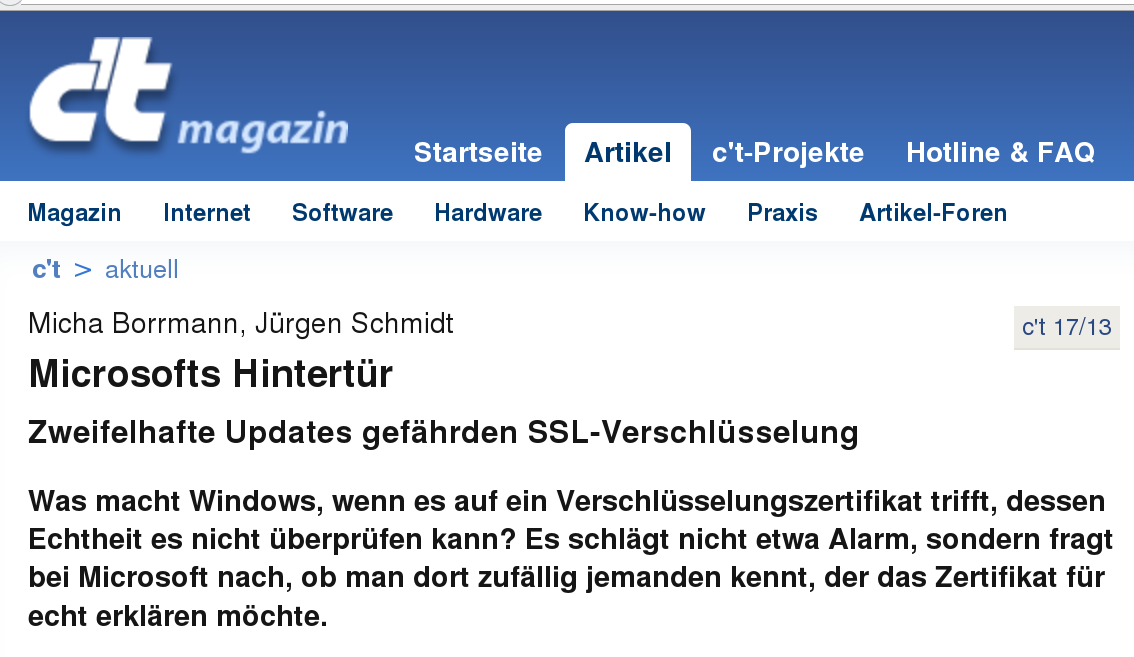
\includegraphics[width=10cm]{img/backdoor-windows}
  \par\end{center}
\end{frame}

\begin{frame}
  \frametitle{Backdoors in Windows}
  \begin{center}
    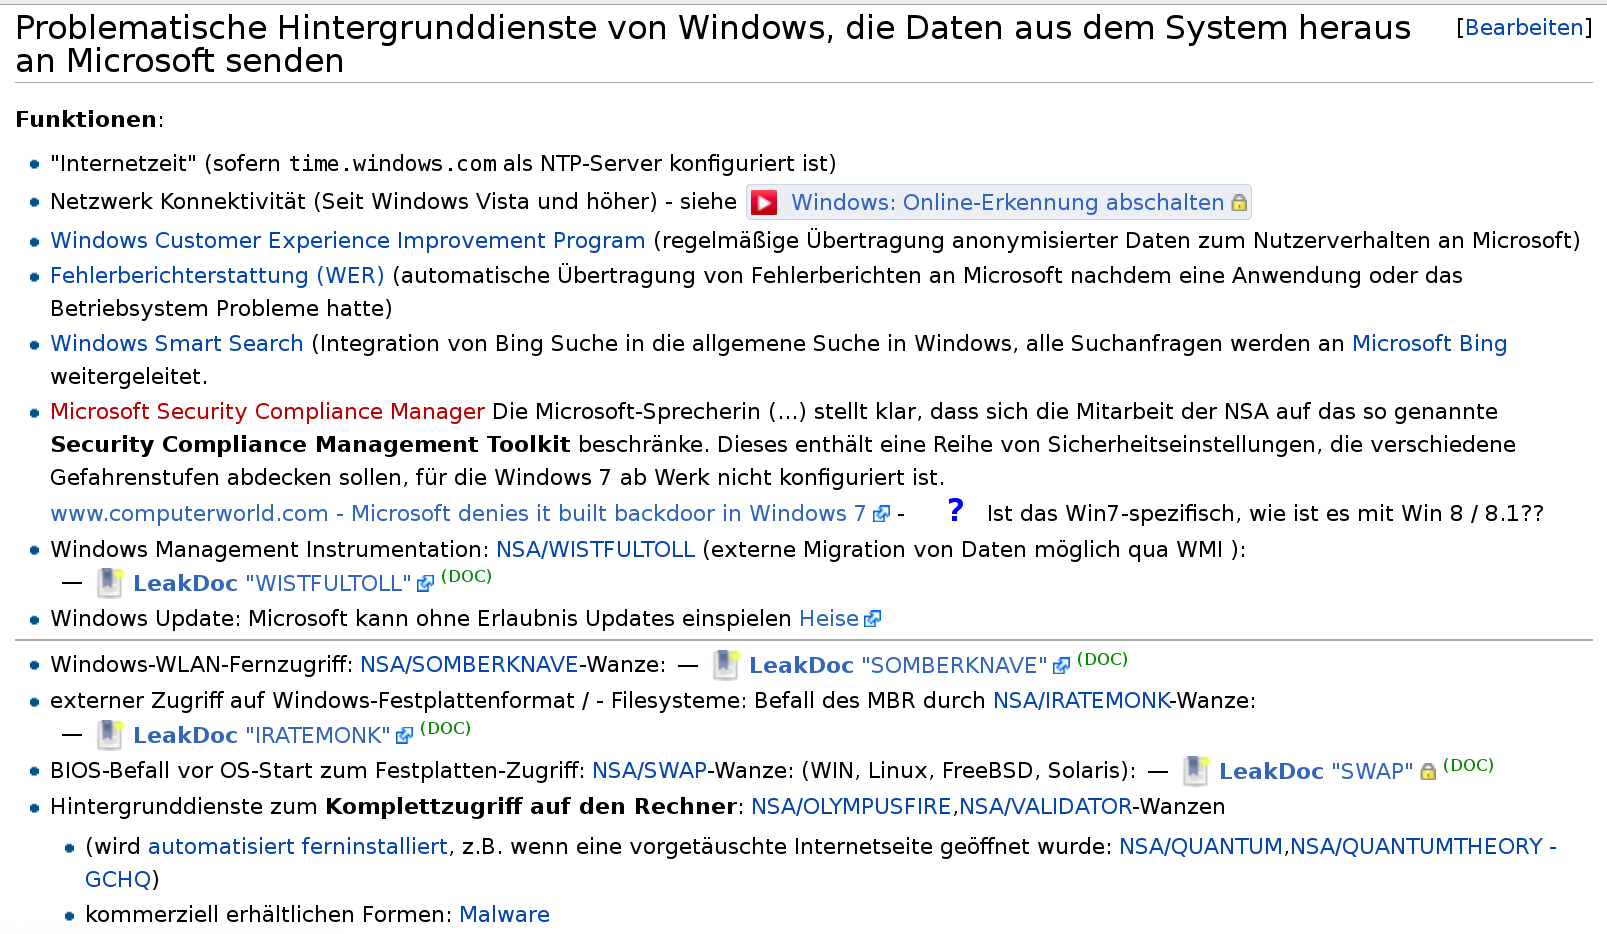
\includegraphics[width=10cm]{img/backdoor-windows2}
  \par\end{center}
\end{frame}

\begin{frame}
  \frametitle{Backdoors in iOS}
  \begin{center}
    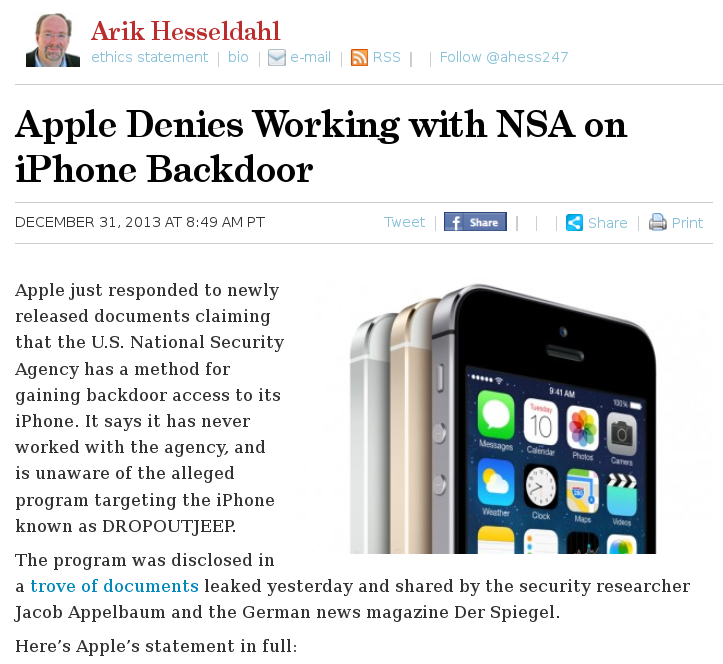
\includegraphics[width=7cm]{img/backdoor-ios}
  \par\end{center}
\end{frame}

\begin{frame}
  \frametitle{Backdoors in Apps}
  \begin{center}
    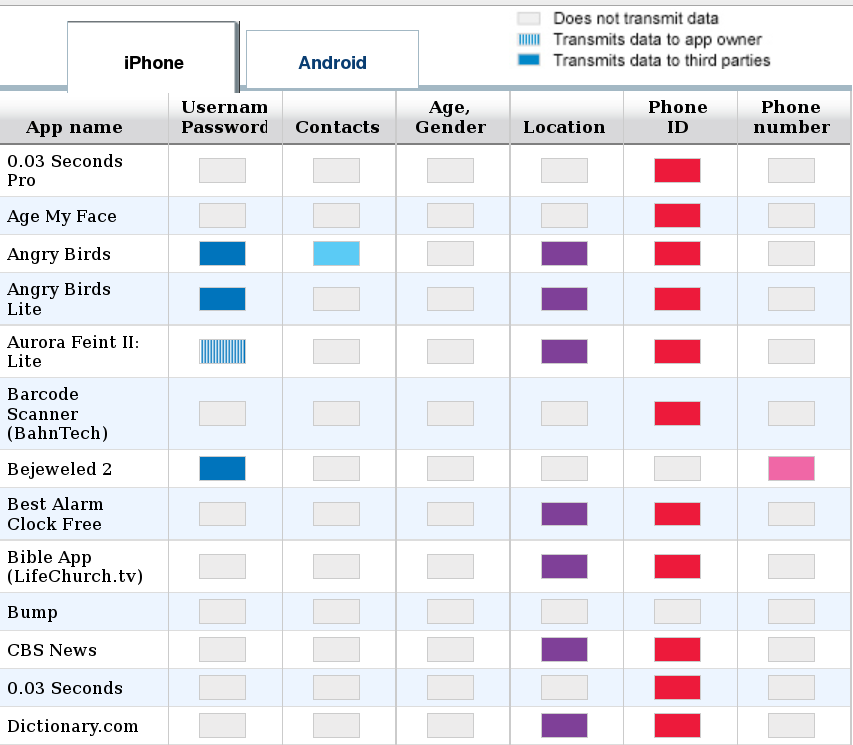
\includegraphics[width=7cm]{img/backdoor-apps}
  \par\end{center}
\end{frame}

\begin{frame}
  \frametitle{Backdoors in Android}
  \begin{center}
    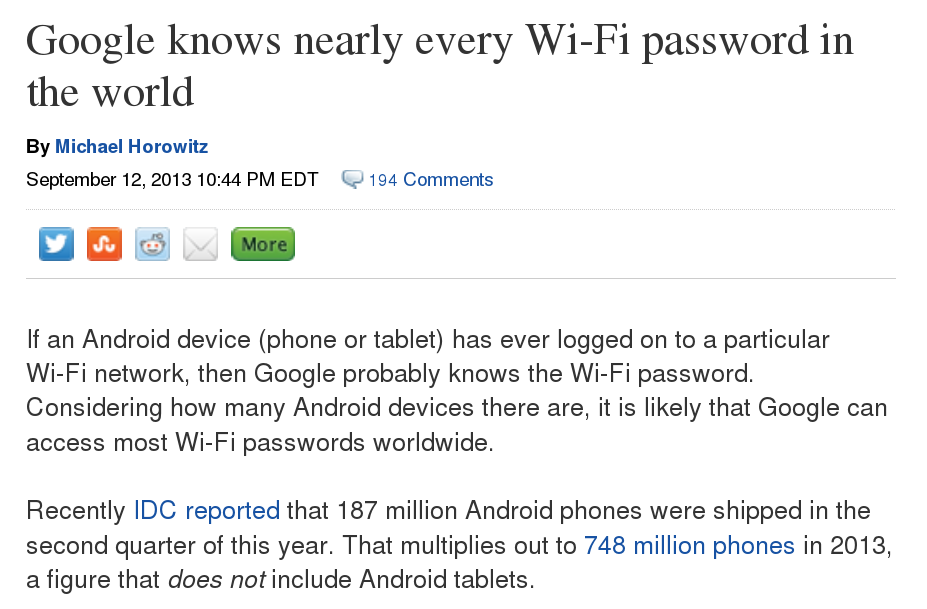
\includegraphics[width=10cm]{img/backdoor-android}
  \par\end{center}
\end{frame}

\begin{frame}
  \frametitle{Backdoors in Apps}
  \begin{center}
    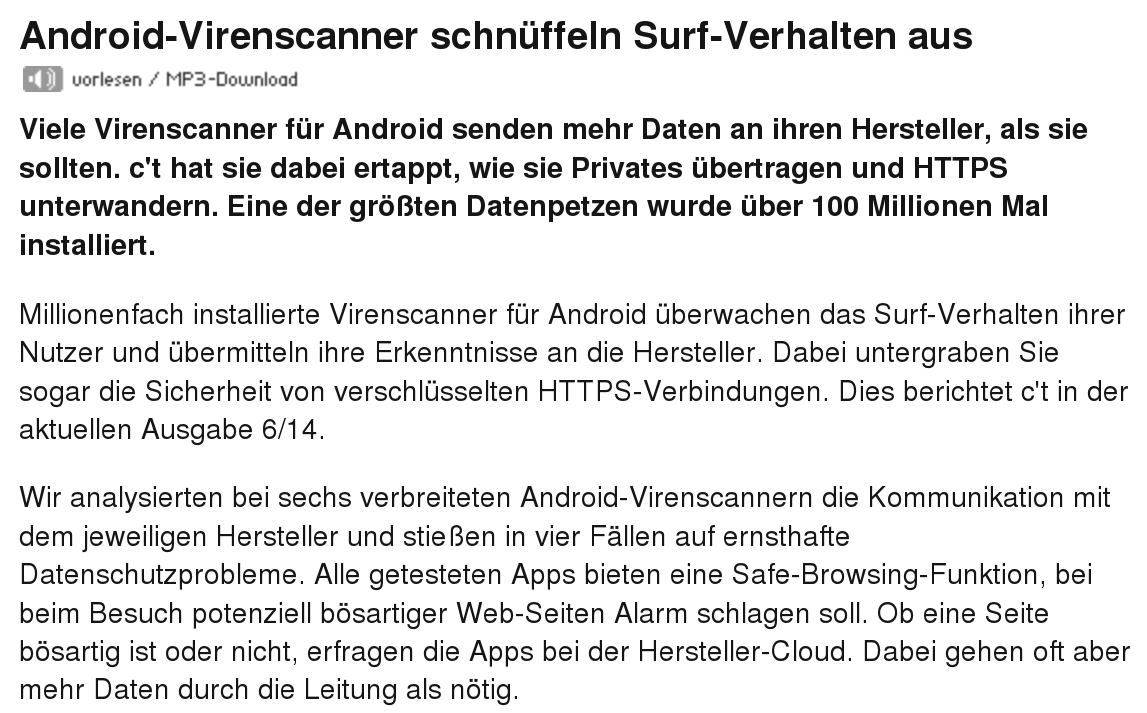
\includegraphics[width=10cm]{img/backdoor-av}
  \par\end{center}
\end{frame}

\begin{frame}
  \frametitle{Backdoors in Apps}
  \begin{center}
    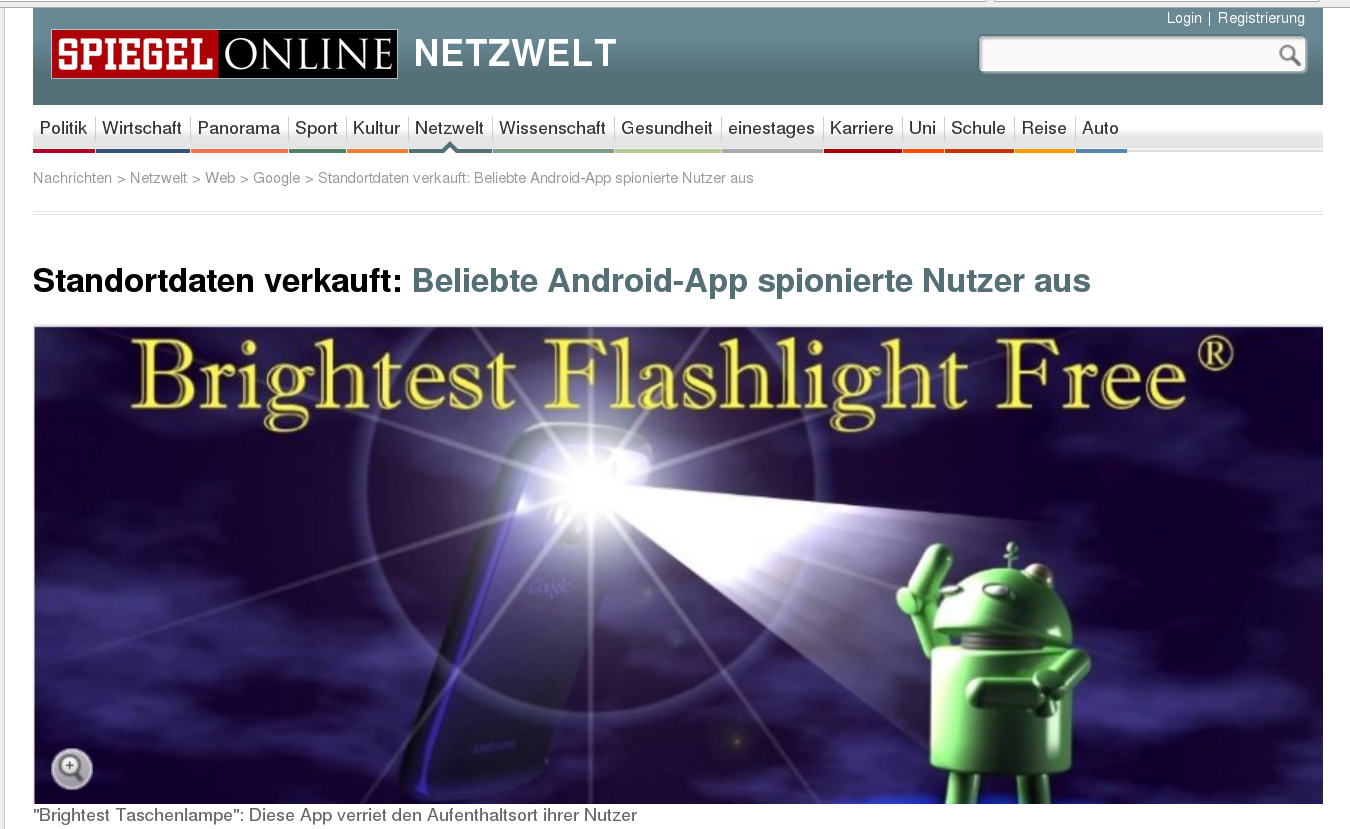
\includegraphics[width=10cm]{img/backdoor-flashlight}
  \par\end{center}
\end{frame}

\begin{frame}
  \frametitle{Backdoors in Apps}
  \begin{center}
    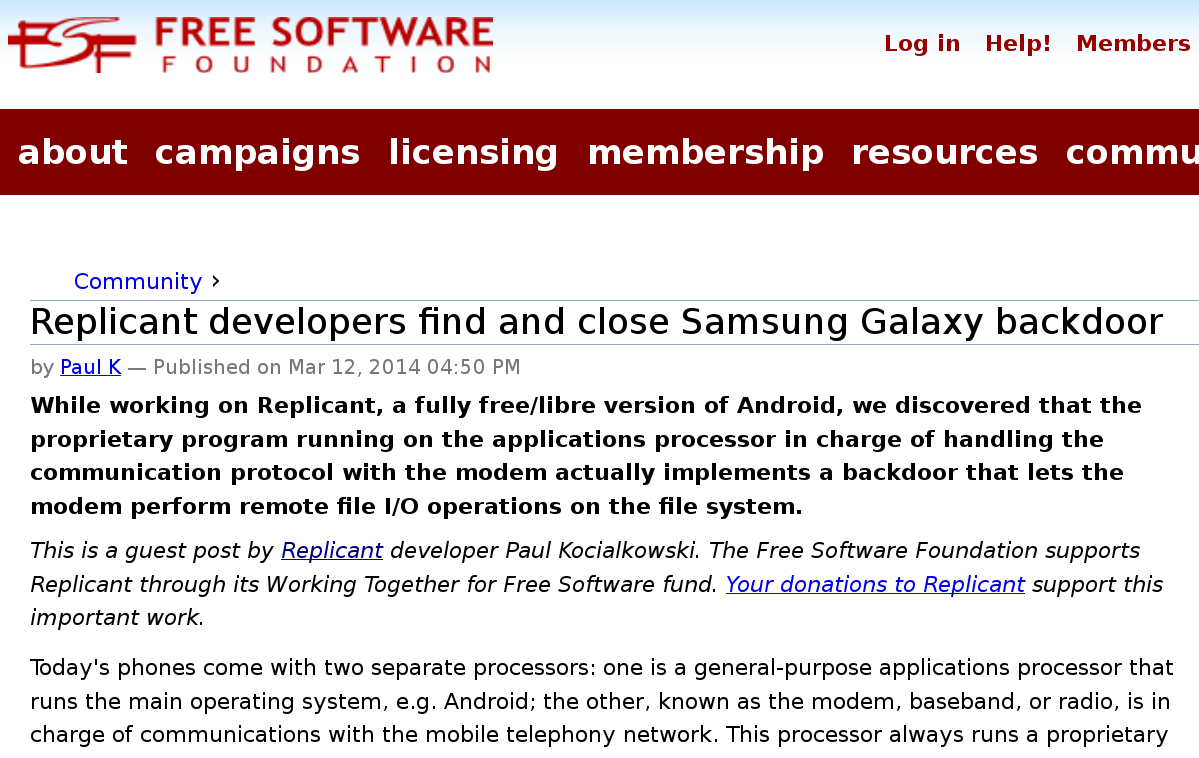
\includegraphics[width=10cm]{img/backdoor-samsung}
  \par\end{center}
\end{frame}

\begin{frame}
  \frametitle{Backdoors in Apps}
  \begin{center}
    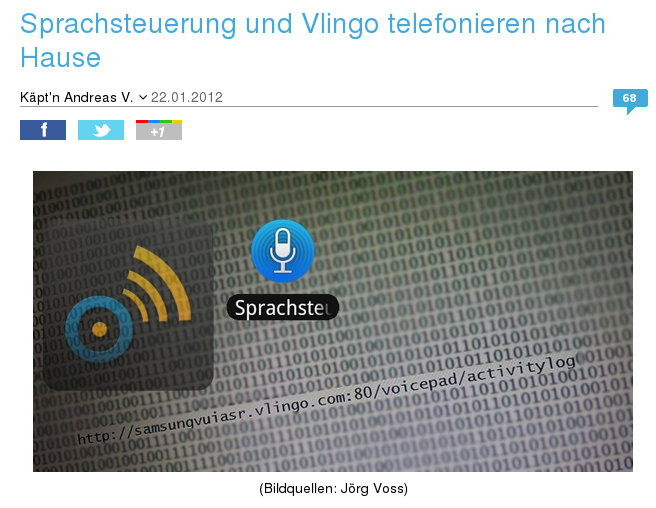
\includegraphics[width=8cm]{img/backdoor-samsung2}
  \par\end{center}
\end{frame}

\begin{frame}{Das GNU Projekt}
  \begin{columns}
    \column{6cm}

    \begin{itemize}
      \item Begonnen von Richard Stallman im Jahr 1984 
      \item Gründung der Free Software Foundation im Jahr 1985 
    \end{itemize}

    \column{7cm}

    \begin{center}
      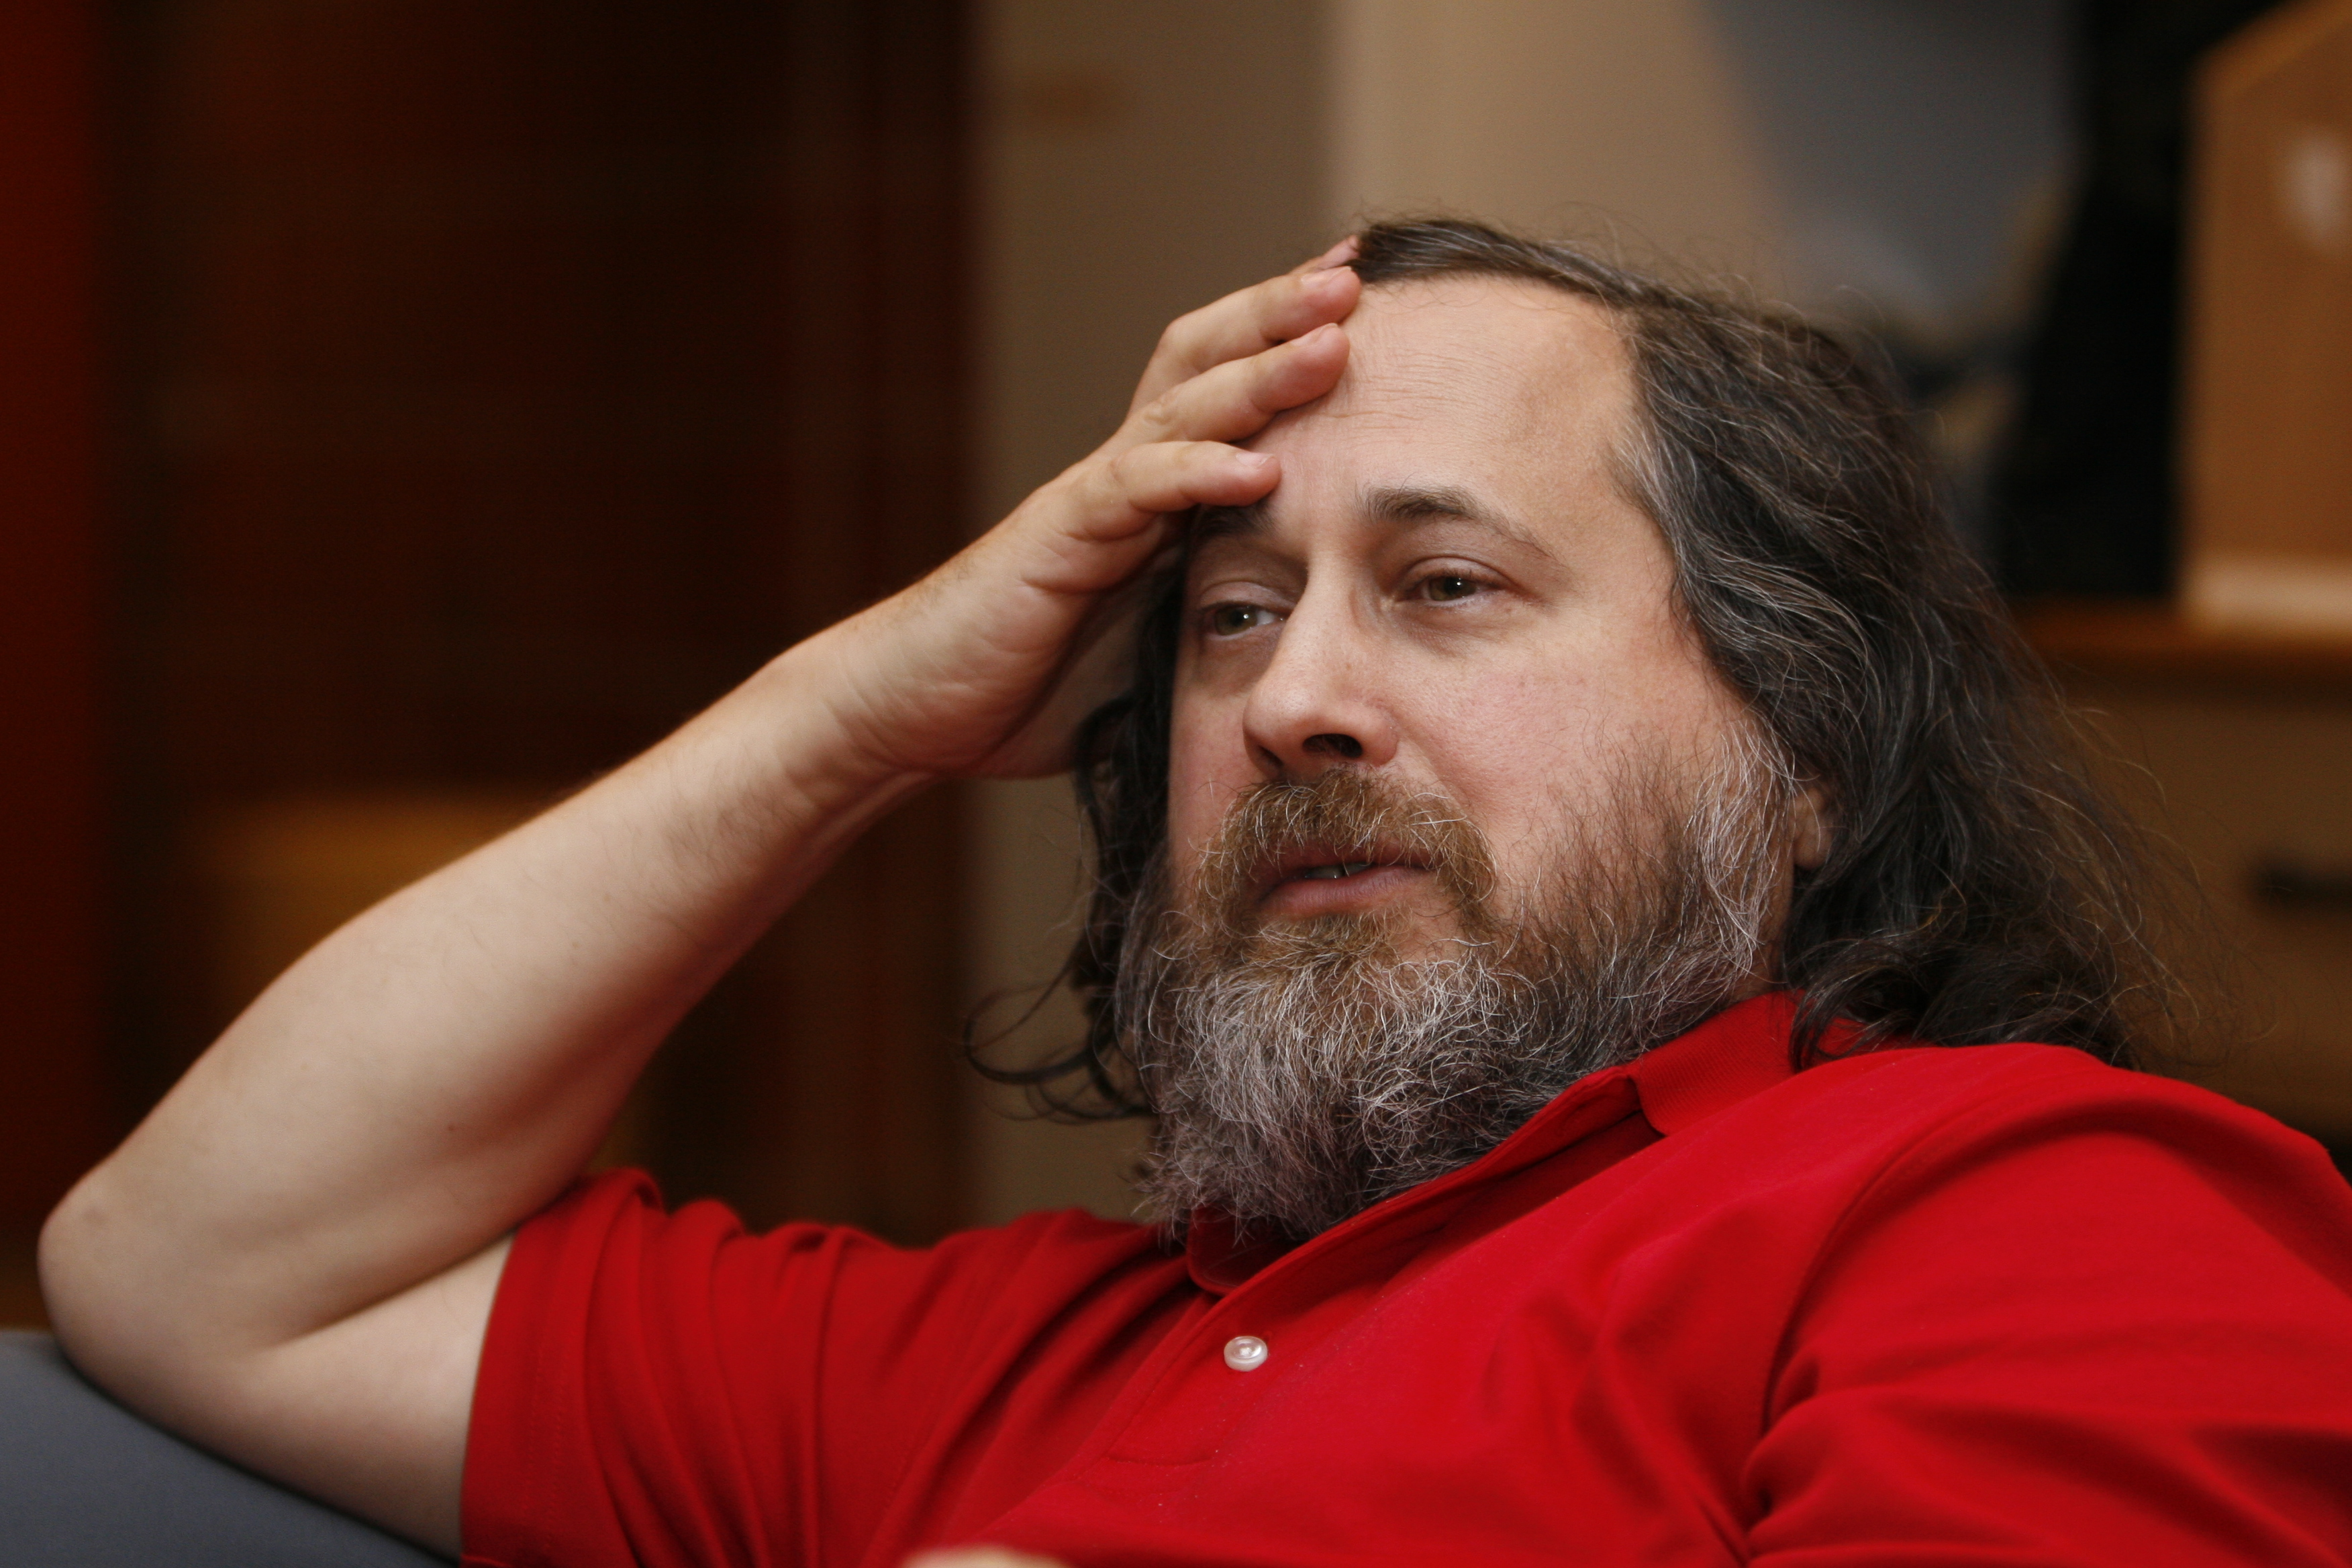
\includegraphics[width=4.5cm]{img/stallman}
    \par\end{center}

    \begin{center}
      
\includegraphics[width=5cm]{img/logo-fsf}
    \par\end{center}
  \end{columns}
\end{frame}

\begin{frame}{LibreOffice}
  \begin{columns}
    \column{6cm}

    \begin{itemize}
      \item Textverarbeitung
      \item Tabellenkalkulation
      \item Präsentationen
      \item Formeleditor
      \item nutzt Open Document Format zur Speicherung
    \end{itemize}

    \column{5cm}

    \begin{center}
      
\includegraphics[width=5cm]{img/LibreOffice}
    \par\end{center}
  \end{columns}
\end{frame}

\begin{frame}{Freie Software für Android}
  \begin{columns}
    \column{6cm}

    \textbf{F-Droid}
    \begin{itemize}
      \item Installationsdienst für freie Android-Software
    \end{itemize}

    \vspace{0.5cm}

    \textbf{TextSecure}
    \begin{itemize}
      \item Verschlüsselter Nachrichtenaustausch
      \item Verschlüsselte Speicherung
    \end{itemize}

    \column{5cm}

    \begin{center}
      \includegraphics[width=2cm]{img/F-Droid_Logo_2}
    \par\end{center}
    \begin{center}
      \includegraphics[width=2cm]{img/TextSecure_Icon}
    \par\end{center}
  \end{columns}
\end{frame}

\begin{frame}{Replicant}
  \begin{columns}
    \column{6cm}
    \begin{itemize}
      \item basiert auf Android
      \item Ziel, alle proprietären Komponenten durch freie zu ersetzen
      \item Einbindung von F-Droid
      \item \textbf{Problem:} Verlust der Garantie bei Installation
    \end{itemize}
    \column{5cm}
    \begin{center}
      \includegraphics[width=2cm]{img/Replicant_logo_alpha}
    \par\end{center}
  \end{columns}
\end{frame}

\begin{frame}{Linux}
  \begin{columns}
    \column{8cm}
    \begin{itemize}
      \item Weit verbreitet als Server-Betriebssystem
      \item Bekannte Desktop-Varianten: 

      \begin{itemize}
        \item Ubuntu/Debian Linux
        \item OpenSUSE
      \end{itemize}
      \item Können als Live-System ausprobiert werden
      \item Integrierte Software für Verschlüsselung, Webbrowsing, E-Mail, Textverarbeitung
      etc.
    \end{itemize}
    \column{6cm}

    \begin{center}
      \includegraphics[width=3cm]{img/Tux}
    \par\end{center}
  \end{columns}
\end{frame}

\begin{frame}
  \frametitle{Linux}
  \begin{center}
    \includegraphics[width=10cm]{img/gnome}
  \par\end{center}
\end{frame}

\section{Verhalten}
\subsection{}

\begin{frame}
    \frametitle{Datensparsamkeit}
    \begin{itemize}
        \item<2-> Viele Daten zusammen ergeben Profile
        \item<3-> Werden die Daten gebraucht?
        \item<4-> Werden echte Daten gebraucht?
            \begin{itemize}
              \item<5-> Pseudonymität
              \item<6-> mailinator.com (Wegwerf-Email-Adresse)
	      \item<7-> frank-geht-ran.de (Wegwerf-Telefonnummer)
              \item<8-> bugmenot.com (Fake Accounts)
            \end{itemize}
    \end{itemize}
\end{frame}

\begin{frame}
    \frametitle{Passwörter}
    \begin{itemize}
        \item<2-> Keine einfachen Wörter
        \item<3-> Groß-, Kleinbuchstaben, Ziffern, Sonderzeichen
        \item<4-> Beispiele:
            \begin{itemize}
                \item<5-> dragon
                \item<6-> (nCuAj.§Tsm!f
                \item<7-> IchLiebeDich
                \item<8-> .§)=/)=`
                \item<9-> qwerty
                \item<10-> Mks?o/.u,1Psw!
            \end{itemize}
        \item<12-> Verschiedene Passwörter nutzen!
        \item<13-> Passwort-Manager verwenden \\ (z.B. Keepass, Password Safe)
    \end{itemize}
\end{frame}

\begin{frame}
  \frametitle{Diskussion}
  \begin{center}
    {\Large Diskussion}\\
    \vspace{5mm} 
    \href{https://github.com/c3d2/cms-nsa}{Folien}: \href{https://creativecommons.org/licenses/by-sa/4.0/}{\cc{by-sa}} Chaos Computer Club Dresden \\
    \vspace{4mm}
    CMS Dresden: schule@c3d2.de
  \end{center}
\end{frame}

\end{document}
